% File: CableTension1.tex
% Author: Adam Leeper
%------------------------------------------------------------------------------
\providecommand{\isolatedBuild}[1]{#1}% Fallback definition to build normally.
\isolatedBuild{
  \documentclass[11pt,letterpaper]{book}
  %\documentclass[11pt,letterpaper]{book}

% aleeper: I think these are needed for Paul's macros?
\usepackage{epsfig}
\usepackage{epstopdf}

%\makeatletter
%\typeout{The import path is \import@path}
%\makeatother

\usepackage{import}

\subimport{./}{packagesMitiguy.sty}
\subimport{./}{macrosMitiguy.tex}
\subimport{./}{PageStylesMitiguy.tex}
\subimport{./}{macrosLeeper.tex}
   % Found via TEXINPUTS environment variable.
  \isolatedBuildHeader{Vector Basics: Unit Vectors and Cross Product}
                      {Calculating Moments Using Cross Product}
                      %\footnote{Adapted from problem 3.2.38 of Sheri Sheppard's textbook.}}
}
%%%
%%%
%%%
\begin{minipage}[t]{0.6\linewidth}
  \minipageTopAnchor
  (Adapted from problem 3.2.38 of Sheri Sheppard's textbook.)
  %
  \\[0.45pc]
  The figure at right shows a cable connected to a lever.
  The tension in the cable is $T = \SI{610}{\newton}$.
  Determine the moment about point $O$ created by the force of the cable
  acting on the lever. Express your answer in terms of unit vectors
  \uvecHat{x}, \uvecHat{y}, and \uvecHat{z} which are directed along the axes shown.
\end{minipage}
\begin{minipage}[t]{0.4\linewidth}
  \minipageTopAnchor
  \centering
  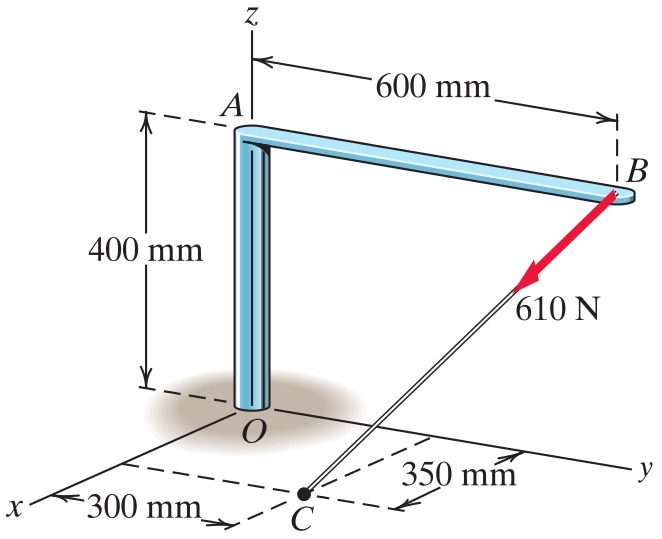
\includegraphics[width=5cm]{sheppard_3-2-38.jpg}
\end{minipage}
%
\\[0.45pc]
\Solution{}{0.97\linewidth}{
  We'll denote the force applied at point $B$ as $\force{B}$.
  Using the \textit{definition}, the moment of this force about point $O$ is:
  $$\moment{\force{B}/O} \deff[\;] \posvec{O}{B} \CrossProduct[\;] \force{B}$$
  %
  %Let's form each ingredient.
  %\\[0.45pc]
  \textbf{Position vector:} The position vector is formed by direct
  inspection of the figure. If this is not obvious to you, place your finger
  at $O$ and trace a path to $B$, writing down the distance and direction you
  moved at each step.
  %
  %\\[0.45pc]
  %\begin{tabular}{lcl}
    $$\posvec{O}{B} \equals[\;] \posvec{O}{A} \plus[\;] \posvec{A}{B}
      \equals[\;] 400~\si{mm} ~\uvecHat{z} \plus[\;] 600~\si{mm}~\uvecHat{y}$$
  %\end{tabular}
  %
  %\\[0.45pc]
  \textbf{Force vector:} We are given the tension in the cable, so we know the
  magnitude of the force is \SI{610}{\newton}.
  We do not know the direction, but we have geometric information in the
  figure we can use to find the direction. The line of action of the
  force passes through points $B$ and $C$, so to form the force we need the
  unit vector from $B$ to $C$, denoted $\uvecFromTo{B}{C}$.
  %
  $$\force{B} \equals[\;] T ~\uvecFromTo{B}{C} \equals[\;]
    T \frac{\posvec{B}{C}}{\magnitude{\posvec{B}{C}}}$$
  %
  As before, we find \posvec{B}{C} by inspection:
  $$\posvec{B}{C}
    \equals[\;] \posvec{O}{C} \plus[\;] \posvec{B}{O}
    \equals[\;] (350 ~\uvecHat{x} \plus[\;]  300 ~\uvecHat{y}) \plus[\;]
                (-600 ~\uvecHat{y} \plus[\;] -400 ~\uvecHat{z})
    \equals[\;]  350~\si{mm}~\uvecHat{x} \plus[\;] -300~\si{mm}~\uvecHat{y}
                 \plus[\;] -400~\si{mm}~\uvecHat{z}$$
  And we find the magnitude from the definition:
  $$\vectorMagnitudeDefinition{\posvec{B}{C}} \equals[\;]
    \underbrace{
      \sqrt{(350~\si{mm})^2 \plus[\;] (-300~\si{mm})^2 \plus[\;]
            (-400~\si{mm})^2
           }
    }_\text{(Valid for vector expressed in a single,
             unitary orthogonal basis.)}
    \equals[\;] 610.3~\si{mm}$$
%  \begin{align*}
%    \magnitude{\posvec{B}{C}}
%    & \deff[\;] \vectorMagnitudeExpression{\posvec{B}{C}}
%    \\[0.45pc]
%    & \equals[\;] \sqrt{
%        ( 350)^2 ~\cancelto{1}{\uvecHat{x} \DotProduct[\;] \uvecHat{x}} \plus[\;]
%        (-300)^2 ~\cancelto{1}{\uvecHat{y} \DotProduct[\;] \uvecHat{y}} \plus[\;]
%        (-400)^2 ~\cancelto{1}{\uvecHat{z} \DotProduct[\;] \uvecHat{z}}}
%    & \text{(Only valid for single, unitary orthogonal basis.)}
%    \\[0.45pc]
%    & \equals[\;] 610.328 \text{~mm}
%  \end{align*}
  Hence, the force vector is
  $$\force{B} \equals[\;] T ~\uvecFromTo{B}{C} \equals[\;]
    (610~\si{\newton})~
    \frac{(350~\si{mm}~\uvecHat{x} \plus[\;]
          -300~\si{mm} ~\uvecHat{y} \plus[\;] -400~\si{mm} ~\uvecHat{z})}
         {610.3~\si{mm}}
    \approx 350~\si{\newton}~\uvecHat{x} \plus[\;]
           -300~\si{\newton}~\uvecHat{y} \plus[\;]
           -400~\si{\newton}~\uvecHat{z}.$$
  %
  Finally, we have the ingredients to compute the moment:
  %
  \begin{center}
  \begin{tabular}{l@{}c@{}l}
    $\moment{\force{B}/O}$ & $\deff[\;]$
    & $\posvec{O}{B} \CrossProduct[\;] \force{B}$
    \\[0.45pc]
    & $\equals[\;]$
    & $(600~\si{mm}~\uvecHat{y} \plus[\;] 400~\si{mm}~\uvecHat{z})
       \CrossProduct[\;]
       (350~\si{\newton}~\uvecHat{x} \plus[\;] -300~\si{\newton}~\uvecHat{y}
       \plus[\;] -400~\si{\newton}~\uvecHat{z})$
    \\[0.45pc]
    & $\equals[\;]$
    & $(~(600)(350) \cancelto{-\uvecHat{z}}{\uvecHat{y} \CrossProduct[\;] \uvecHat{x}} \plus[\;]
         (600)(-300)\cancelto{\zerovec    }{\uvecHat{y} \CrossProduct[\;] \uvecHat{y}} \plus[\;]
         (600)(-400)\cancelto{+\uvecHat{x}}{\uvecHat{y} \CrossProduct[\;] \uvecHat{z}} \plus[\;]$
    \\[0.45pc]
    &
    & $~~(400)(350) \cancelto{+\uvecHat{y}}{\uvecHat{z} \CrossProduct[\;] \uvecHat{x}} \plus[\;]
         (400)(-300)\cancelto{-\uvecHat{x}}{\uvecHat{z} \CrossProduct[\;] \uvecHat{y}} \plus[\;]
         (400)(-400)\cancelto{\zerovec    }{\uvecHat{z} \CrossProduct[\;] \uvecHat{z}} ~)~
         \si{\newton.\mm}$
    \\[0.45pc]
    & $\equals[\;]$
    & $(-120,000~\uvecHat{x} \plus[\;] 140,000~\uvecHat{y} \plus[\;] -210,000~\uvecHat{z})
        ~\si{\newton\mm}$
    \\[0.45pc]
    & $\equals[\;]$
    & $(-120~\uvecHat{x} \plus[\;] 140~\uvecHat{y} \plus[\;] -210~\uvecHat{z})
        ~\si{\newton\m}$
  \end{tabular}
  \end{center}
}

\Solution{}{0.97\linewidth}{
  %
  \textbf{Addendum:}
  A force is applied at a specific \textit{physical} point of a body, which
  is why moments are defined using a position vector to the point of application.
  However, \textit{mathematically} we can use any point that is on the force's
  ``line of action". In some problems this can dramatically simplify the math.
  %
  \\[0.45pc]
  In this problem the math isn't any simpler, but we can show that picking the
  point on the ground gives us the same result as before
  (note the use of the equal sign; this is \underline{not} a definition):
  %
  \begin{center}
  \begin{tabular}{l@{}c@{}l}
    $\moment{\force{B}/O}$ & $\equals[\;]$
    & $\posvec{O}{C} \CrossProduct[\;] \force{B}$
    \\[0.45pc]
    & $\equals[\;]$
    & $(350~\si{mm}~\uvecHat{x} \plus[\;] 300~\si{mm}~\uvecHat{y})
       \CrossProduct[\;]
       (350~\si{\newton}~\uvecHat{x} \plus[\;] -300~\si{\newton}~\uvecHat{y}
       \plus[\;] -400~\si{\newton}~\uvecHat{z})$
    \\[0.45pc]
    & $\equals[\;]$
    & $(~(350)(350) \cancelto{\zerovec    }{\uvecHat{x} \CrossProduct[\;] \uvecHat{x}} \plus[\;]
         (350)(-300)\cancelto{+\uvecHat{z}}{\uvecHat{x} \CrossProduct[\;] \uvecHat{y}} \plus[\;]
         (350)(-400)\cancelto{-\uvecHat{y}}{\uvecHat{x} \CrossProduct[\;] \uvecHat{z}} \plus[\;]$
    \\[0.45pc]
    &
    & $~~(300)(350) \cancelto{-\uvecHat{z}}{\uvecHat{y} \CrossProduct[\;] \uvecHat{x}} \plus[\;]
         (300)(-300)\cancelto{\zerovec    }{\uvecHat{y} \CrossProduct[\;] \uvecHat{y}} \plus[\;]
         (300)(-400)\cancelto{+\uvecHat{x}}{\uvecHat{y} \CrossProduct[\;] \uvecHat{z}} ~)~
         \si{\newton.\mm}$
    \\[0.45pc]
    & $\equals[\;]$
    & $(-120,000~\uvecHat{x} \plus[\;] 140,000~\uvecHat{y} \plus[\;] -210,000~\uvecHat{z})
        ~\si{\newton\mm}$
    \\[0.45pc]
    & $\equals[\;]$
    & $(-120~\uvecHat{x} \plus[\;] 140~\uvecHat{y} \plus[\;] -210~\uvecHat{z})
        ~\si{\newton\m}$
  \end{tabular}
  \end{center}
}
%
\isolatedBuildFooter
